\subsection{Datasets}
\par We studied 20 datasets, including 8 undirected graphs and 12 directed graphs. The details of the graphs are shown below.

\begin{table}[h]
\fontsize{8}{10}\selectfont
\begin{tabular}{lllll}
Dataset        & File                         & Category      & Directed & Description                            \\ \hline
skitter        & as-skitter.ungraph-75000.txt & Physical      & N        & autonomous systems on web              \\
Caida          & as-Caida.undir.txt           & Physical      & N        & autonomous systems on web              \\
Enron          & email-Enron.ungraph.txt      & Communication & N        & email records between employees        \\
EU institution & email-EuAll.txt              & Communication & Y        & email records between employees        \\
Amazon         & com-amazon.ungraph-75000.txt & Co-occurence  & N        & bought X also bought Y                 \\
DBLP           & com-dblp.ungraph-75000.txt   & Coauthorship  & N        & coauthorship relationship              \\
astro-ph       & ca-AstroPh.txt               & Coauthorship  & Y        & coauthorship relationship              \\
Protein        & bio-protein-undir.txt        & Metabolic     & N        & metabolic interaction between proteins \\
JDK            & soft-jdkdependency.txt       & Software      & Y        & dependency between Java classes        \\
Spanish book   & text-spanishbook.txt         & Lexical       & Y        & word following relationship            \\
Gnutella       & p2p-Gnutella31.txt           & Computer      & Y        & connection between hosts               \\
hep-ph         & cit-HepPh.txt                & Citation      & Y        & citation relationship                  \\
hep-th         & cit-HepTh.txt                & Citation      & Y        & citation relationship                  \\
cora           & cit-Cora.txt                 & Citation      & Y        & citation relationship                  \\
Hamsterster    & soc-hamsterster.undir.txt    & Social        & N        & social network friendship              \\
Youtube        & soc-Youtube-75000.undir.txt  & Social        & N        & social network friendship              \\
Slashdot       & soc-Slashdot0811-75000.txt   & Social        & Y        & directed friend/foe relationship       \\
digg           & soc-digg.txt                 & Social        & Y        & reply from one user to another         \\
flickr         & soc-flickr-75000.txt         & Social        & Y        & directed friendship                    \\
pokec          & soc-pokec-75000.txt          & Social        & Y        & directed friendship                                       \\ \hline
\end{tabular}
\end{table}

In the following sections, we present our analysis on common features and distinctive patterns among these 20 dataset for various graph algorithms. Specifically, these algorithms include degree distributions, PageRank, weakly connected components, K-Core connected components with k=5, eigendecomposition and triangle count.

\subsection{Degree distributions}
\begin{figure}[H]
\begin{center}
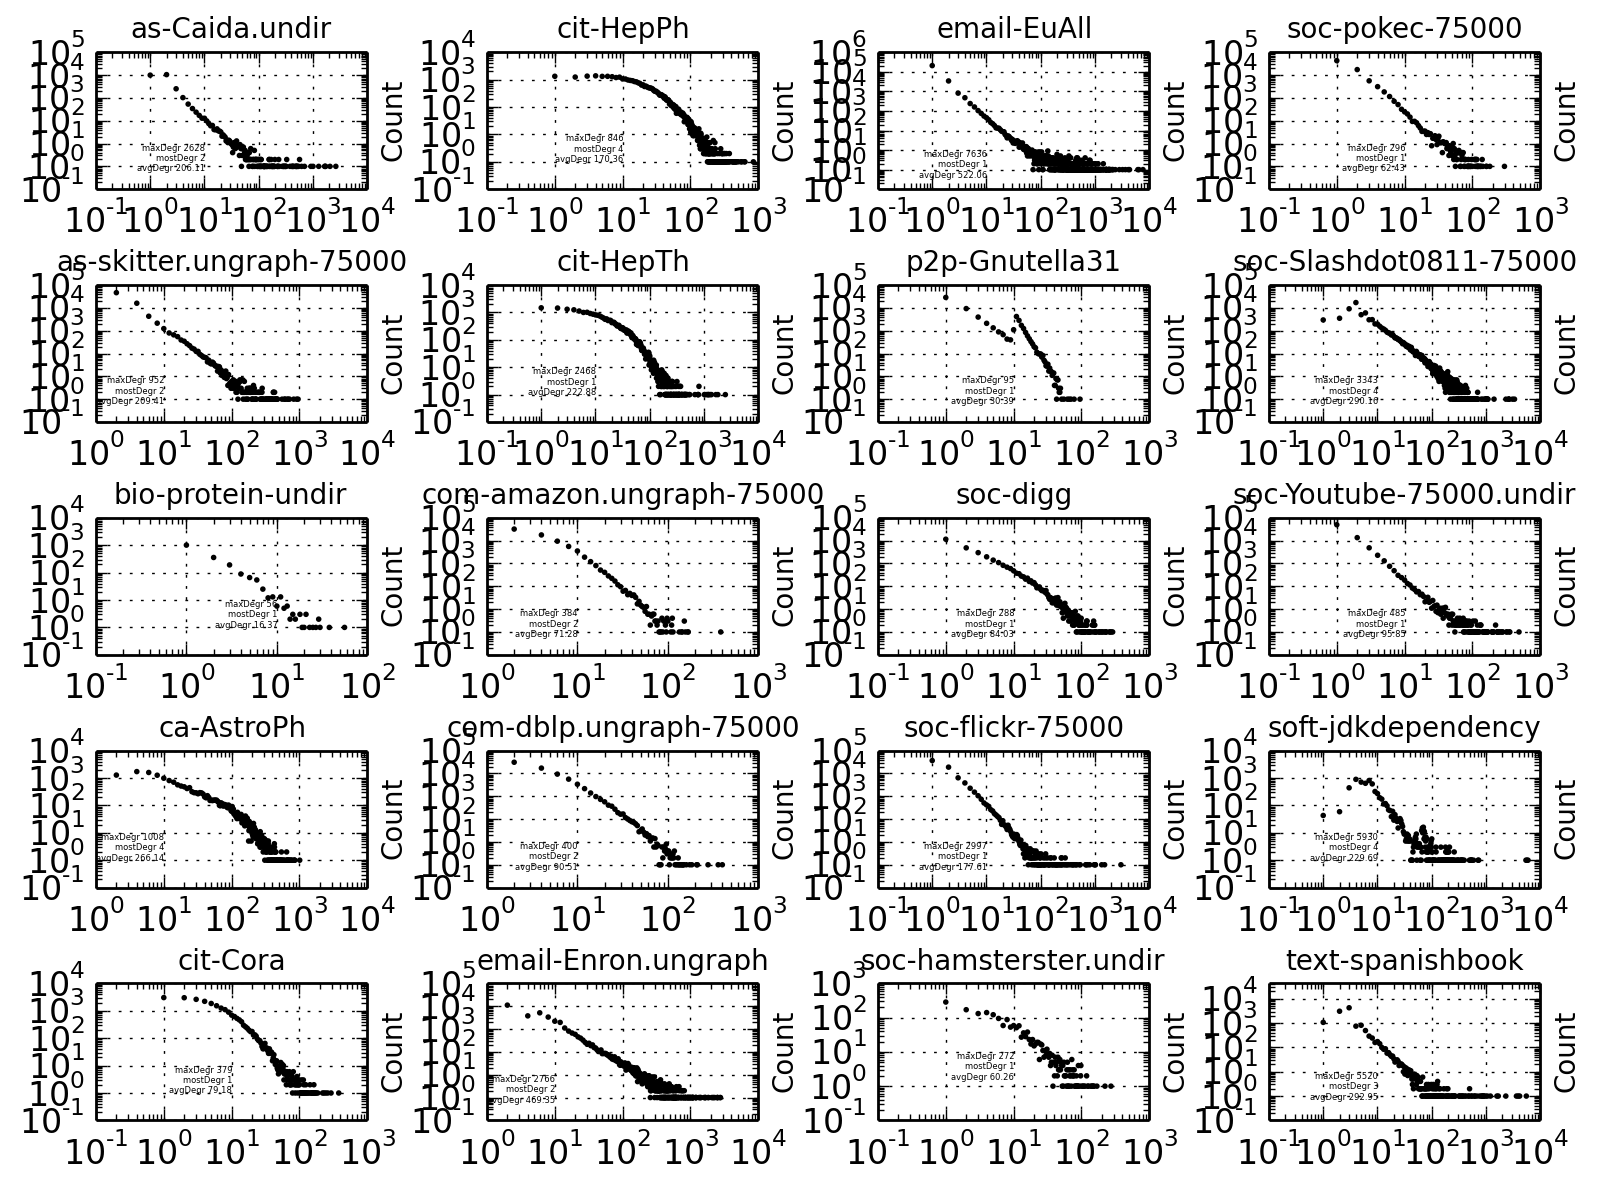
\includegraphics[width=\textwidth]{FIG/degreedist.png} 
\end{center}
\end{figure}
\subsection{PageRank}
\subsection{Weakly connected components}
\subsection{K-Core connected components with k=5}
\subsection{Eigendecomposition}
\subsection{Triangle count}